% Options for packages loaded elsewhere
\PassOptionsToPackage{unicode}{hyperref}
\PassOptionsToPackage{hyphens}{url}
\documentclass[
  12pt,
  a4paper]{extarticle}
\usepackage{xcolor}
\usepackage[margin=2.5cm]{geometry}
\usepackage{amsmath,amssymb}
\setcounter{secnumdepth}{5}
\usepackage{iftex}
\ifPDFTeX
  \usepackage[T1]{fontenc}
  \usepackage[utf8]{inputenc}
  \usepackage{textcomp} % provide euro and other symbols
\else % if luatex or xetex
  \usepackage{unicode-math} % this also loads fontspec
  \defaultfontfeatures{Scale=MatchLowercase}
  \defaultfontfeatures[\rmfamily]{Ligatures=TeX,Scale=1}
\fi
\usepackage{lmodern}
\ifPDFTeX\else
  % xetex/luatex font selection
\fi
% Use upquote if available, for straight quotes in verbatim environments
\IfFileExists{upquote.sty}{\usepackage{upquote}}{}
\IfFileExists{microtype.sty}{% use microtype if available
  \usepackage[]{microtype}
  \UseMicrotypeSet[protrusion]{basicmath} % disable protrusion for tt fonts
}{}
\makeatletter
\@ifundefined{KOMAClassName}{% if non-KOMA class
  \IfFileExists{parskip.sty}{%
    \usepackage{parskip}
  }{% else
    \setlength{\parindent}{0pt}
    \setlength{\parskip}{6pt plus 2pt minus 1pt}}
}{% if KOMA class
  \KOMAoptions{parskip=half}}
\makeatother
\usepackage{longtable,booktabs,array}
\usepackage{calc} % for calculating minipage widths
% Correct order of tables after \paragraph or \subparagraph
\usepackage{etoolbox}
\makeatletter
\patchcmd\longtable{\par}{\if@noskipsec\mbox{}\fi\par}{}{}
\makeatother
% Allow footnotes in longtable head/foot
\IfFileExists{footnotehyper.sty}{\usepackage{footnotehyper}}{\usepackage{footnote}}
\makesavenoteenv{longtable}
\usepackage{graphicx}
\makeatletter
\newsavebox\pandoc@box
\newcommand*\pandocbounded[1]{% scales image to fit in text height/width
  \sbox\pandoc@box{#1}%
  \Gscale@div\@tempa{\textheight}{\dimexpr\ht\pandoc@box+\dp\pandoc@box\relax}%
  \Gscale@div\@tempb{\linewidth}{\wd\pandoc@box}%
  \ifdim\@tempb\p@<\@tempa\p@\let\@tempa\@tempb\fi% select the smaller of both
  \ifdim\@tempa\p@<\p@\scalebox{\@tempa}{\usebox\pandoc@box}%
  \else\usebox{\pandoc@box}%
  \fi%
}
% Set default figure placement to htbp
\def\fps@figure{htbp}
\makeatother
\setlength{\emergencystretch}{3em} % prevent overfull lines
\providecommand{\tightlist}{%
  \setlength{\itemsep}{0pt}\setlength{\parskip}{0pt}}
\newcommand{\BOO}{BOO}
\usepackage{float}
\usepackage{bookmark}
\IfFileExists{xurl.sty}{\usepackage{xurl}}{} % add URL line breaks if available
\urlstyle{same}
\hypersetup{
  pdftitle={ClavertonDown Example},
  pdfauthor={Emma Cliffe, Skills Centre: MASH, University of Bath},
  hidelinks,
  pdfcreator={LaTeX via pandoc}}

\title{ClavertonDown Example}
\author{Emma Cliffe, Skills Centre: MASH, University of Bath}
\date{August 2020}

\usepackage{amsthm}
\theoremstyle{plain}
\newtheorem*{theorem*}{Theorem}\newtheorem{theorem}{Theorem}[section]
\theoremstyle{definition}
\newtheorem*{definition*}{Definition}\newtheorem{definition}{Definition}[section]
\theoremstyle{plain}
\newtheorem*{proposition*}{Proposition}\newtheorem{proposition}[theorem]{Proposition}
\newtheorem*{Definitions*}{Definitions}\newtheorem{Definitions}[definition]{Definitions}
\theoremstyle{plain}
\newtheorem*{lemma*}{Lemma}\newtheorem{lemma}{Lemma}[section]
\theoremstyle{plain}
\newtheorem*{corollary*}{Corollary}\newtheorem{corollary}{Corollary}[section]
\theoremstyle{plain}
\newtheorem*{conjecture*}{Conjecture}\newtheorem{conjecture}{Conjecture}[section]
\theoremstyle{definition}
\newtheorem*{example*}{Example}\newtheorem{example}{Example}[section]
\theoremstyle{definition}
\newtheorem*{exercise*}{Exercise}\newtheorem{exercise}{Exercise}[section]
\newtheorem*{Thought*}{Thought}\newtheorem{Thought}{Thought}[section]
\theoremstyle{remark}
\newtheorem*{remark*}{Remark}
\newtheorem*{solution*}{Solution}
\newtheorem*{Example*}{Example}
\theoremstyle{remark}
\newtheorem*{Proof*}{Proof}
\newtheorem*{Examples*}{Examples}
\let\BeginKnitrBlock\begin \let\EndKnitrBlock\end


%\usepackage[english,shorthands=off]{babel}
\usepackage{etoolbox}
\usepackage{spverbatim}
\makeatletter
\@ifpackageloaded{float}{}{\usepackage{float}}
\@ifpackageloaded{adjustbox}{}{\usepackage[Export]{adjustbox}}
\makeatother
\floatplacement{figure}{H}
\newcommand{\scalefactor}{1.2}
\adjustboxset*{min width=\scalefactor\width,max width=\linewidth}
\renewcommand{\familydefault}{phv}
\fontfamily{phv}\selectfont
\renewcommand{\em}{\bf}\renewcommand{\textit}{\textbf}\renewcommand{\emph}{\textbf}\renewcommand{\it}{\bf}\renewcommand{\itshape}{\bf}
\setlength{\parindent}{0.0pt}
\setlength{\parskip}{1.0\baselineskip}
\renewcommand{\baselinestretch}{1.5}\selectfont
\setlength{\mathsurround}{0.2em}
\setlength{\arraycolsep}{0.5cm}\renewcommand{\arraystretch}{1.5}
\addtolength{\jot}{\baselineskip}
\renewcommand{\;}{\,}
\sloppy
\allowdisplaybreaks
\usepackage{amsthm}
\newtheoremstyle{plain}{20pt}{3pt}{}{}{\bfseries}{.\newline\nobreak}{1.0em\nobreak}{}
\newtheoremstyle{definition}{20pt}{3pt}{}{}{\bfseries}{.\newline\nobreak}{1.0em\nobreak}{}
\newtheoremstyle{remark}{20pt}{3pt}{}{}{\bfseries}{.\newline\nobreak}{1.0em\nobreak}{}
\csundef{Proof}
\csundef{endProof}
\newenvironment{Proof}
  {\noindent{\bf Proof.}\hspace*{1em}}% Begin
  {\qed\par}% End
%% When redefining an environment it is vital that it has 
%% the same number of arguments as the original
\renewenvironment{proof}[1][\proofname]
  {\trivlist\item\relax\noindent{\bf {#1}.}\hspace*{1em}}% Begin
  {\qed\endtrivlist}% End

\begin{document}
\maketitle

{
\setcounter{tocdepth}{2}
\tableofcontents
}
\newpage
\pagenumbering{arabic}

\section*{Introduction}\label{introduction}
\addcontentsline{toc}{section}{Introduction}

ClavertonDown is aimed at staff at the University of Bath which is located on Claverton Down. It uses knitr, RMarkdown and Bookdown and aims to produce a system for creating sets of lecture notes in a variety of formats, including those which are technically accessible and those which are often preferred by disabled students. We aim for the system to be usable in both pure and applied mathematical settings. Requests to adapt the system or the outputs of the system to meet these goals will be considered by MASH. The main contact email address is \href{mailto:mash-access@bath.ac.uk}{\nolinkurl{mash-access@bath.ac.uk}} but you should use the Team set up by the Centre for Learning and Teaching for support in the first instance.

This document is \textbf{also} a work in progress. Like everything right now!

\section{What formats do I need to produce and why?}\label{what-formats-do-i-need-to-produce-and-why}

ClavertonDown can produce:

\begin{itemize}
\tightlist
\item
  HTML book
\item
  HTML page
\item
  Standard, clear and large print PDF
\item
  Word document
\item
  EPub book
\end{itemize}

From a technical point of view only three of these formats of mathematical text are accessible:

\begin{itemize}
\tightlist
\item
  HTML using MathJax to render all mathematical text (HTML book and page)

  \begin{itemize}
  \tightlist
  \item
    HTML formats must meet WCAG 2.1 Level AA requirements and use MathJax to render all mathematical text.
  \item
    You can check your document meets the legal requirement of WCAG 2.1 Level AA with e.g.~\href{https://accessibilityinsights.io/docs/en/web/overview}{Accessibility Insights for Web plugin for Chrome}
  \item
    You can check it is MathJax by right clicking on the expression (try it in the HTML version):
    \[x = \frac{-b\pm\sqrt{b^2 - 4ac}}{2a}\]
  \end{itemize}
\item
  Word document using in-built Equation Editor for all mathematical text

  \begin{itemize}
  \tightlist
  \item
    Word formats must pass the in-built Accessibility Checker and use the in-built Equation Editor for all mathematical text.
  \item
    You can use the in-built Word Accessibility Checker and information on \href{https://support.office.com/en-gb/article/make-your-word-documents-accessible-to-people-with-disabilities-d9bf3683-87ac-47ea-b91a-78dcacb3c66d}{Making your Word documents accessible} to check your document.
  \item
    You can use Review -\textgreater{} Read Aloud (Alt + Ctrl + Space) to check the maths
  \end{itemize}
\item
  EPub3 using MathML for all mathematical text:

  \begin{itemize}
  \tightlist
  \item
    If the HTML format is accessible then the EPub3 output from ClavertonDown will be also
  \end{itemize}
\end{itemize}

The output from ClavertonDown will meet these requirements as far as possible. However, we cannot stop you from doing things which will fail to meet requirements. In particular, if you use images, sound, videos, colour or interactive/dynamic elements within the HTML you will need to ensure that you have done so within the accessibility requirements.

\subsection{Why do we still supply inaccessible PDFs?}\label{why-do-we-still-supply-inaccessible-pdfs}

It isn't possible to create accessible PDFs using LaTeX. Even if a PDF is accessible the mathematical text within it will \textbf{still be technically inaccessible} regardless of how the PDF has been produced but\ldots{}

\begin{itemize}
\tightlist
\item
  not all accessibility is about technical access - for some a clear or large print PDF is best
\item
  currently, clear print is selected most often by disabled students in the Department of Mathematical Sciences
\item
  PDF remains the best fallback when a student is concerned that a document is not being rendered as the author intended
\item
  PDF remains the best starting point for creating hard copy resources which is important for some disabled students
\end{itemize}

Finally, our aim here is to produce choice for \emph{all} students, disabled or not, and many will still select PDF.

\subsection{Do I really have to put all this on Moodle?}\label{do-i-really-have-to-put-all-this-on-moodle}

If you use the same set up as this example document then all the outputs will be collected together into a single folder. We recommend that you:

\begin{itemize}
\tightlist
\item
  Zip up the folder and upload it to Moodle \emph{as a file}
\item
  Select Add a resource -\textgreater{} File. Give the resource a name (e.g.~lecture notes 1).
\item
  Add the zip file. Right click on the zip file, a window appears, click on unzip and wait until complete.
\item
  Right click on the zip again and click on delete. You will have a folder remaining.
\item
  Left click on the folder to open it.
\item
  Find the main file index.html and right click on this,
  a window appears, click on Set main file.
\item
  Change any other settings you wish in the resource and then save.
\end{itemize}

When you click on this resource you will see the HTML book version of the notes. This is technically accessible, searchable and usable on a mobile device. In the menu at the top there is a download button, from here a student can access any of the other formats. This is as close as we can get to replicating the Blackboard Ally student experience of being able to transform accessible resources to other formats.

\section{Theorems and stuff}\label{theorems-and-stuff}

You will notice that there are a variety of ways that theorem type environments are presented in the different formats. All of these pass technical accessibility tests or are following RNIB Clear Print guidelines and have been used for at least a decade in our provision for disabled students. We have also take on feedback that in HTML formats colour might be helpful to show where environments start and finish. We have chosen to impose a structured colour scheme on you, for now. The colours have been chosen so that they pass accessibility tests for contrast with the text.

However, this doesn't mean we have got it right. Give us feedback. Ideally, get students to give feedback too.

\BeginKnitrBlock{theorem}[Foo]
{\label{thm:thm1} }
This is a theorem environment already provided by Bookdown. It still works as before.
\EndKnitrBlock{theorem}

\BeginKnitrBlock{proposition}[Thingy we need for \ref{thm:thm1}]
{\label{prp:prp1} }
However, in this system you can now

\begin{itemize}
\tightlist
\item
  Change the numbering system of the inbuilt environments - this is done in the file \_bookdown.yml. Please see the file in the same folder as this file.
\item
  Reference other environments within names. Notice that you need to use a double backslash.
\end{itemize}
\EndKnitrBlock{proposition}

\BeginKnitrBlock{Proof*}[Of theorem \ref{thm:thm1}]
{}
You can make new unnumbered theorem environments. You can call them whatever you like. They work kind of like the inbuilt ones but the environment is always newtheorem and the env defines the type.

You need to have predefined the type and made any changes to the standard print style in the file \_bookdown.yml. Please see the file in the same folder as this file.

You can't control what things look like in the other formats as they have been designed with a variety of accessibility features. If you don't like how they look then maybe contact us and ask about it. It might be something we can think about changing or allowing author control or, it might not.
\qed
\EndKnitrBlock{Proof*}

\BeginKnitrBlock{proof}[Proof of theorem \ref{thm:thm1}]
Defining your own proof environment doesn't stop the inbuilt one working.
\EndKnitrBlock{proof}

\BeginKnitrBlock{definition}
{\label{def:unnamed-chunk-3} }
You can leave some things numbered on their own.
\EndKnitrBlock{definition}

\BeginKnitrBlock{Definitions}
{\label{Def:def1}}
You can create new numbered theorem types. Unlike inbuilt environments, for them to be numbered in all formats they \emph{must} have a label. If you forget then they won't be numbered in any format \emph{except} for PDF and then your numbering won't match. I might try and fix this at some point. You can number them alone or with other inbuilt or newtheorem environments.

You need to have predefined the type, the numbering and made any changes to the standard print style in the file \_bookdown.yml. Please see the file in the same folder as this file.

Take care not to reuse the inbuilt numbering labels with your new theorems! This will lead to odd things happening. The inbuilt labels to avoid are: thm, lem, cor, prp, cnj, def, exm, exr, fig, tab and eq.
\EndKnitrBlock{Definitions}

References still work in the same way as in Bookdown. Now go to theorem \ref{thm:thm1} or proposition \ref{prp:prp1}.

Here is some text which is not part of the below example.
\BeginKnitrBlock{Examples*}
{}You can turn off the colour and padding in html, ePub and Word for any newtheorem or inbuilt theorem type. You do this in the \_bookdown.yml file by adding the theorem name to the colouroff style\_with list.
\EndKnitrBlock{Examples*}
Here is some text which is not part of the above example.

\subsection{But I want to number some of them\ldots{}}\label{but-i-want-to-number-some-of-them}

\BeginKnitrBlock{Definitions*}
{}This is unnumbered in all formats
\EndKnitrBlock{Definitions*}

\BeginKnitrBlock{Definitions}
{\label{Def:def3}}This should be definitions 2.3 in all formats
\EndKnitrBlock{Definitions}

\subsubsection{Out of interest\ldots{}}\label{out-of-interest}

What happens if I try to number an environment I have specifically declared to be unnumbered? e.g.~using \{newtheorem, env=`Examples', label=``argh''\}

This will fail to compile for PDF and it will produce ``Examples (\#Examples:argh)'' as the title in other formats.

The only real benefit to be gained from specifically declaring an environment to be unnumbered is that you are less likely to accidentally number an instance of it!

\subsection{Colour has meaning}\label{colour-has-meaning}

The coloured styles for theorem-type environments in HTML, EPub and Word are an attempt to colour code based very broadly on the mathematical type of enviroment. This is to respond to feedback that clear visual markers of the start and end of theorems was important. For accessibility purposes the use of colour can also be used to facilitate cognitive processing and this is stronger if the choice of colour has meaning.

LaTeX styling, while originally intended to broadly correspond to semantic type is, in our decade or so of experience, not used this way by authors of lecture notes due to the fonts and styling which are imposed in standard LaTeX. So, the three styles in LaTeX:

\begin{itemize}
\tightlist
\item
  Plain
\item
  Definition
\item
  Remark
\end{itemize}

are used to impose the authors visual preferences mostly with respect to font, font attributes and layout. That is, they are usually syntactic choices, not semantic ones.

Hence, our assignment is NOT based, at all, on the PDF styling specified by the author, or any other information like e.g.~numberwith.

Since the user can define any number of new theorem type environments we have to\ldots{} guess\ldots{} to try and align colours to broad types. We have four HTML styles:

\begin{itemize}
\tightlist
\item
  ProofStyle: (P\textbar p)roof(s), (S\textbar s)olution(s), (S\textbar s)oln(s), (R\textbar r)emark(s) and anything including these words; if not then one of the below
\item
  ExampleStyle: (E\textbar e)xample(s), (E\textbar e)xercise(s) and anything including these words; if not then one of the below
\item
  DefinitionStyle: (D\textbar d)efinition(s), (D\textbar d)efn(s) and anything including these words; if not then defaults to the below
\item
  TheoremStyle: Everything else - but should definitely include (T\textbar t)heorem(s), (L\textbar l)emma(s), (C\textbar c)orollar(y\textbar ies), (P\textbar p)roposition(s), (C\textbar c)onjecture(s).
\end{itemize}

You might find this automatic sorting to be wrong or annoying. Also, we can't possibly guess what you might call things so lots of types which aren't theorem-like will end up with the default theorem colouring which isn't helpful.

This is an accessibility issue - the use of colour to highlight meaning helps with processing so we need to give you control to an extent.

\subsubsection{So\ldots?}\label{so}

We have given the author direct control over which class of HTML to place each theorem type in - both in built and new theorems. You can override our guesses. We have also given you control to turn off italics in the book HTML (the other accessible formats have this turned off already).

\begin{itemize}
\tightlist
\item
  To turn off italics change style\_with -\textgreater{} italicsoff to TRUE in the \_bookdown.yml file (or add this to a file you already have). You don't need to specify this, if you don't, for backwards compatibility, it will default to italicsoff is FALSE
\item
  To classify theorem types you can add, if you wish, a classify\_as section to your \_bookdown.yml. Again, you don't need to add this if you don't want to change anything. You can see an example of this in the \_bookdown.yml file for this document in which the new theorem type Thought is classified as an example. If you remove this classification it will default to the theorem type and the below will change colour.
\end{itemize}

\BeginKnitrBlock{Thought*}
{}Here is a thought.
\EndKnitrBlock{Thought*}

\section{Figures inside other environments}\label{figures-inside-other-environments}

\subsection{Here is a figure}\label{here-is-a-figure}

\begin{figure}
\centering
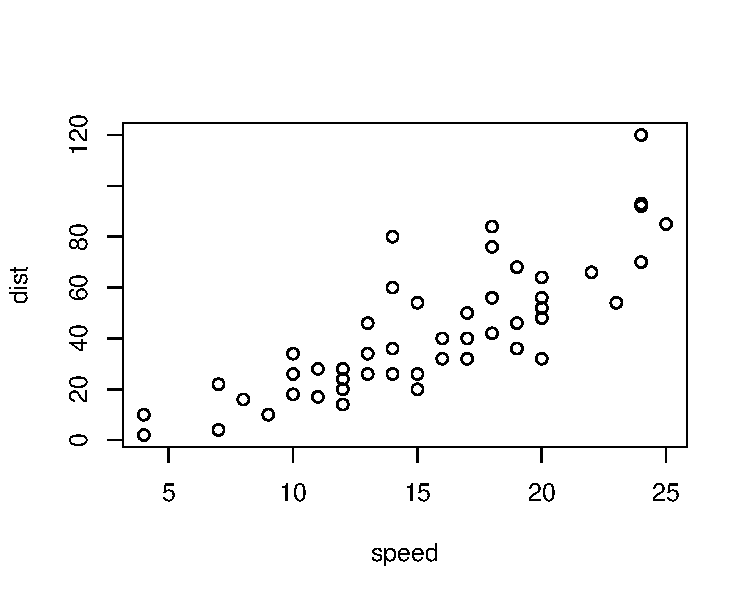
\includegraphics[width=0.6\linewidth,height=\textheight,keepaspectratio]{./Notes_files/figures/cars-plot-1.pdf}
\caption{\label{fig:cars1}This is title and a caption with a reference \ref{thm:thm1} inside it}
\end{figure}

\subsection{Here is the putting of a figure inside another built in environment}\label{here-is-the-putting-of-a-figure-inside-another-built-in-environment}

\BeginKnitrBlock{example}
{\label{exm:unnamed-chunk-7} }Here is an example.

\begin{figure}
\centering
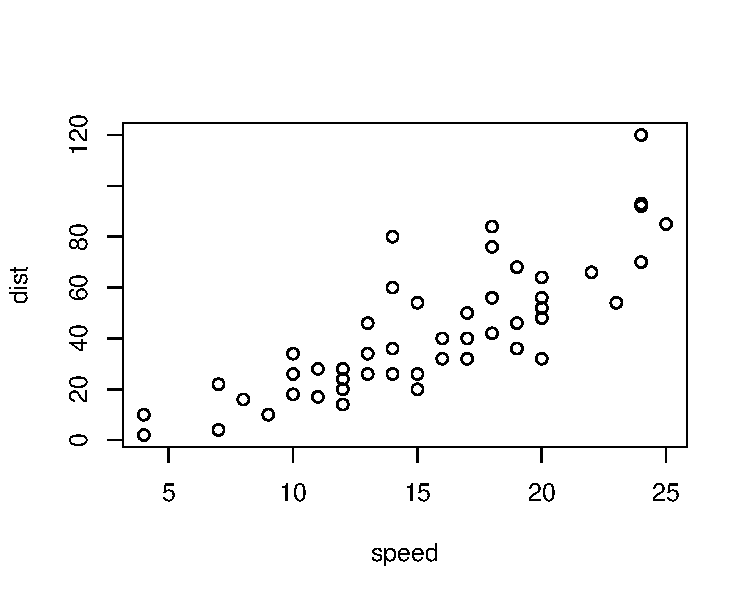
\includegraphics[width=0.6\linewidth,height=\textheight,keepaspectratio]{./Notes_files/figures/cars-plot-1.pdf}
\caption{\label{fig:cars2}Something to do with cars}
\end{figure}

This is a test. So, you need an empty line before and after the above for it to be a float. At the end of an environment this means that you need TWO empty lines. This is Pandoc.
\EndKnitrBlock{example}

\subsection{Here is the putting of a figure inside a newtheorem}\label{here-is-the-putting-of-a-figure-inside-a-newtheorem}

Here we are going to do something a bit more impressive with the automatic creation of alternative image formats. This is only useful to you if you are using R to generate graphs etc.

\BeginKnitrBlock{Example*}
{}An example in which we have autogenerated a useful description of the scatterplot for a person who cannot see it, using BrailleR. To see the content of the long description if you view the HTML in Firefox and right click you can request it.

\begin{figure}
\centering
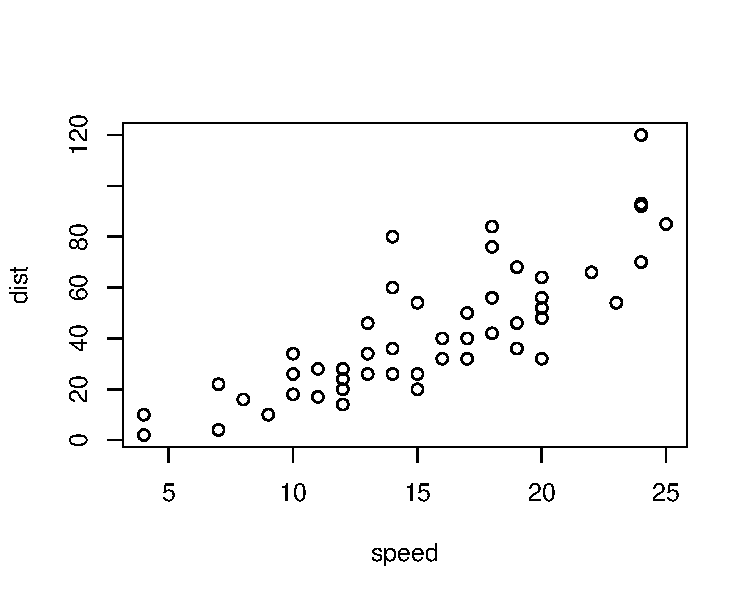
\includegraphics[width=0.6\linewidth,height=\textheight,keepaspectratio]{./Notes_files/figures/cars-plot-1.pdf}
\caption{\label{fig:cars3}More cars things}
\end{figure}
\EndKnitrBlock{Example*}

\section{Repeating environments}\label{repeating-environments}

Sometimes I would like to repeat a definition from earlier and have it numbered the same. This now works as expected in all formats including the numbering of the environment. However, the numbering of \emph{things inside the environment} will probably be wrong so take care. Tell us if this is important to you as it is low priority at the moment.

Inbuilt using own numbering
\begingroup\renewcommand{\thetheorem}{\ref{thm:thm1}}
\BeginKnitrBlock{theorem}[Foo]
{ }
This is a theorem environment already provided by Bookdown. It still works as before.
\EndKnitrBlock{theorem}
\endgroup\addtocounter{theorem}{-1}
Inbuilt using other inbuilt numbering
\begingroup\renewcommand{\thetheorem}{\ref{prp:prp1}}
\BeginKnitrBlock{proposition}[Thingy we need for \ref{thm:thm1}]
{ }
However, in this system you can now

\begin{itemize}
\tightlist
\item
  Change the numbering system of the inbuilt environments - this is done in the file \_bookdown.yml. Please see the file in the same folder as this file.
\item
  Reference other environments within names. Notice that you need to use a double backslash.
\end{itemize}
\EndKnitrBlock{proposition}
\endgroup\addtocounter{theorem}{-1}
Newtheorem using other inbuilt numbering
\begingroup\renewcommand{\thedefinition}{\ref{Def:def1}}
\BeginKnitrBlock{Definitions}
{}
You can create new numbered theorem types. Unlike inbuilt environments, for them to be numbered in all formats they \emph{must} have a label. If you forget then they won't be numbered in any format \emph{except} for PDF and then your numbering won't match. I might try and fix this at some point. You can number them alone or with other inbuilt or newtheorem environments.

You need to have predefined the type, the numbering and made any changes to the standard print style in the file \_bookdown.yml. Please see the file in the same folder as this file.

Take care not to reuse the inbuilt numbering labels with your new theorems! This will lead to odd things happening. The inbuilt labels to avoid are: thm, lem, cor, prp, cnj, def, exm, exr, fig, tab and eq.
\EndKnitrBlock{Definitions}
\endgroup\addtocounter{definition}{-1}
I still need to test the other combinations. Please tell me if it is broken.

\section{But\ldots{} I want it to do\ldots{}}\label{but-i-want-it-to-do}

We have chosen to create a new package instead of adding to Bookdown because we are diverging from what Bookdown was designed to do. This also means that we can mould how this system works to best meet the needs of students and lecturers.

Tell us what to do next. We'll tell you if it is possible and the likely priority!

\section{LaTeX newcommands, usepackages etc.}\label{latex-newcommands-usepackages-etc.}

You can add these in the header-includes part of the code at the start of this file. You cannot pass a filename to this at the moment. If this is a dealbreaker then let me know. This will work in all formats. \emph{All} other ways of adding commands and packages in will not result in the right thing happening in formats other than PDF, as far as I know.
\[
BOO(x)
\]

\section{Great. How do I use this thing?}\label{great.-how-do-i-use-this-thing}

This package is not on CRAN and it is not going to be in the short or medium term. Instead you need to install it directly from github (if you want to know why then get in touch and ask) which means you will need devtools installed and loaded.

\subsection{Installing ClavertonDown}\label{installing-clavertondown}

Once you have devtools you need to load it:

\begin{quote}
library(devtools)
\end{quote}

Then you can install ClavertonDown:

\begin{quote}
install\_github(``BathMASH/ClavertonDown'')
\end{quote}

Obviously, you need an internet connection.

\subsection{Using ClavertonDown for the first time}\label{using-clavertondown-for-the-first-time}

I suggest that you download the files which were used to create this document:

\begin{itemize}
\tightlist
\item
  \url{https://raw.githubusercontent.com/BathMASH/clavertondown/master/example/index.Rmd}
\item
  \url{https://raw.githubusercontent.com/BathMASH/clavertondown/master/example/_bookdown.yml}
\end{itemize}

Put them in a folder together, open index.Rmd in RStudio and use the Knit menu to compile the various formats. If this doesn't work then something is wrong (get in touch Bath people!). The PDF command creates standard print, clear print and large print PDF.

Then\ldots{} read the files.

\subsubsection{Using the command line}\label{using-the-command-line}

If you prefer to compile from the system command line or via a script then commands along the lines of the below will work. You need to run all five to complete the full set of transformations in the example preamble.

\begin{quote}
Rscript -e ``bookdown::render\_book(`index.Rmd',`clavertondown::gitbook\_clav')''
\end{quote}

\begin{quote}
Rscript -e ``bookdown::render\_book(`index.Rmd',`clavertondown::html\_clav')''
\end{quote}

\begin{quote}
Rscript -e ``bookdown::render\_book(`index.Rmd',`clavertondown::pdf\_clav')''
\end{quote}

\begin{quote}
Rscript -e ``bookdown::render\_book(`index.Rmd',`clavertondown::epub\_clav')''
\end{quote}

\begin{quote}
Rscript -e ``bookdown::render\_book(`index.Rmd',`clavertondown::word\_clav')''
\end{quote}

The pdf\_clav command renders standard print, clear print and large print PDF.

\subsection{Moving from Bookdown to ClavertonDown}\label{moving-from-bookdown-to-clavertondown}

If you have been using Bookdown you may find that simply making changes to your preamble, as per the files above, will result in everything working as expected. You can then start using additional ClavertonDown functionality. If you do not use any of it then your content will, at the time of writing, still work in Bookdown if you change your preamble back. However, if you do not wish to use the additional functionality you should consider whether moving to ClavertonDown is the right choice for you - we are diverging from Bookdown and we cannot guarantee ongoing backwards compatibility. You should also consider that Bookdown is changing in ways that ClavertonDown will not and these are explained in the below section.

\subsubsection{Divergence: why simple preamble changes may not have worked}\label{divergence-why-simple-preamble-changes-may-not-have-worked}

If you have written your Bookdown more recently and are using the \href{https://bookdown.org/yihui/bookdown/markdown-extensions-by-bookdown.html\#theorems}{fenced div environments} rather than the \href{https://bookdown.org/yihui/bookdown/markdown-extensions-by-bookdown.html\#theorem-engine}{knitr engine environments} then simple changes to your preamble will not move your theorem type statements to the new format. They will remain in Bookdown format. We won't be `fixing' this because:

\begin{itemize}
\tightlist
\item
  \href{https://bookdown.org/yihui/bookdown/markdown-extensions-by-bookdown.html\#theorem-engine}{Bookdown documents written using this method can only be converted to PDF and HTML formats}. ClavertonDown exists to enable to conversion to a full range of accessible formats to enable any student to access lecture materials. PDF documents containing mathematical expressions can never be technically accessible and HTML format is only technically accessible for some assistive technology users. Whether you generally supply Word and EPub or not you need to be able to create it on request.
\item
  The work we have done to enable extra functionality cannot be delivered via the fenced div approach at this time. It would require all of the functionality to be reimplemented at a completely different point in the conversion and, based on our current understanding, some of the functionality, which was requested by lecturers and students, could not be delivered at this time if at all.
\item
  While we accept the reasoning for the change in Bookdown - that it enables richer content to be included within theorem type environments and has a clearer implementation - we have not had any request to enable the types of richer functionality meant here. Other `missing' things were considered more of a problem for lecture materials. If future requests fall into these categories we will look at whether we can implement them while retaining the current functionality. It is also noted that our implementation of the knitr custom blocks has already diverged from that in Bookdown. While it is not correct to call it cleaner it should be more robust than the original custom block engines.
\end{itemize}

If you have a Bookdown document which uses fenced divs you should consider how important it is to you to move to ClavertonDown. We have supplied a function which you can run to create a copy of your document and attempt to change format - as Bookdown has created a function which goes back the other way. Our function is going in the more challenging direction and so it aims to only make the change when it is `safe' to do so and maintains a complete original copy untouched without the user needing to ensure this. If when you run the function there are warnings you will need to do some work by hand to complete the change. If you are at Claverton Down then we do ask you to get in touch with us and tell us if you are then missing functionality and we will do our best to assist - or, at least, to be clear about what your options are. It is possible to \href{https://bookdown.org/yihui/bookdown/markdown-extensions-by-bookdown.html\#theorem-engine}{transform back the other way} (this is the easier and safer direction) but

\begin{itemize}
\tightlist
\item
  We will have retained a copy of your original files for you so you don't need to worry about this if you immediately change your mind!
\item
  We assume you are transforming for a reason - to use the functionality of ClavertonDown. In this case any transform back will require you to undo any use of our extra functionality.
\end{itemize}

\subsubsection{I want to transform anyway}\label{i-want-to-transform-anyway}

If, having read the above, you wish to try it out then you need to change directory to that containing your document run the following on the R command line:

\begin{quote}
library(``clavertondown'')
\end{quote}

\begin{quote}
intercept\_theorems(``./'')
\end{quote}

Please read the output carefully.

If you receive \emph{any warning} then you have

\begin{itemize}
\tightlist
\item
  nested theorem type fenced div environments or
\item
  \href{https://bookdown.org/yihui/rmarkdown/language-engines.html}{knitr engine blocks} (including but not limited to theorem type) nested in fenced div theorem type environments or
\item
  You have used more than three colons when defining a fenced div despite it not being nested - just set it back to three in this case.
\end{itemize}

Nesting of this kind cannot be converted - theorem type environments cannot be nested in Clavertondown and knitr engine blocks cannot be nested within theorems. You will need to undo the nesting in whatever way makes sense for your content. This type of nesting is a primary example what Bookdown means by `richer content'.

\section{Can I tell people not at Claverton Down about this?}\label{can-i-tell-people-not-at-claverton-down-about-this}

Yes, sure, that is why it is public. But, this is released with no promises and no warranty. Help will only be provided to staff and students of the University of Bath but we might fix bugs or consider suggestions by others.

\end{document}
